
\begin{figure}
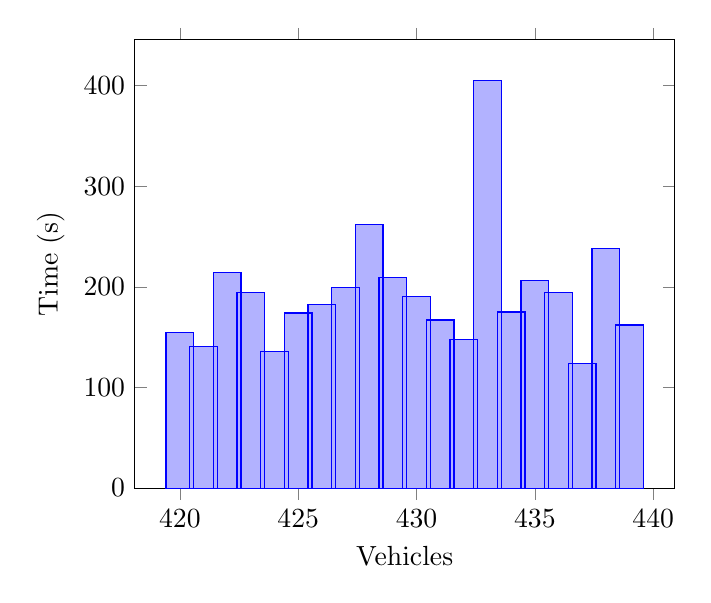
\begin{tikzpicture}
\begin{axis}[
legend style={anchor=west},
xlabel=Vehicles,
ylabel=Time (s),
ymin=0,
ybar,
]
\addplot coordinates {
(421, 141)
(420, 155)
(422, 214)
(427, 199)
(436, 194)
(434, 175)
(435, 206)
(432, 148)
(433, 405)
(430, 190)
(431, 167)
(424, 136)
(439, 162)
(437, 124)
(438, 238)
(429, 209)
(428, 262)
(423, 194)
(425, 174)
(426, 182)
};

\end{axis}
\end{tikzpicture}
\label{tik:time:100:64}
\caption{100 percent diving with GSC on route $64$}
\end{figure}
